\documentclass[a4paper,14pt]{extarticle}
\usepackage[english,russian]{babel}
\usepackage[cache=false]{minted}
\usepackage{fontspec}
\usepackage{indentfirst}
\usepackage{listings}
\usepackage{color}
\usepackage{caption}
\usepackage{amsmath}
\usepackage{hyperref}
\usepackage{graphicx}
\usepackage[%
    left=20mm,%
    right=10mm,%
    top=20mm,%
    bottom=20mm,%
]{geometry}%
\usepackage{titlesec}


\setmainfont{PT Astra Serif}

\hypersetup{
    colorlinks=true,
    linkcolor=black,
    filecolor=magenta,
    urlcolor=cyan,
    pdftitle={Лабораторная работа №4},
    pdfpagemode=FullScreen,
}

\newcommand{\hlink}[2]{\href{#1}{\color{blue}\underline{#2}}}
\graphicspath{ {./images/} }

\setmonofont[Scale=0.8]{JetBrains Mono}
\setminted{frame=lines, framesep=3mm, fontsize=\small}
\usemintedstyle{vs}

\titleformat{\section}
{\normalfont\bfseries}{}{0pt}{Упражнение \thesection.\;}

\titleformat{\subsection}
{\normalfont\bfseries}{}{0pt}{Задание \thesubsection.\;}

\numberwithin{figure}{section}

\begin{document}

\begin{titlepage}
    \vspace{0pt plus2fill}
    \noindent

    \vspace{0pt plus6fill}
    \begin{center}
        \textbf{\large{Санкт-Петербургский национальный исследовательский университет информационных
                технологий, механики и оптики}}

        \vspace{0pt plus2fill}
        \textbf{\Large{ЛАБОРАТОРНАЯ РАБОТА №4}}

        \vspace{0pt plus2fill}
        \textbf{\large{Создание и использование методов}}
    \end{center}

    \vspace{0pt plus8fill}
    \begin{flushright}
        Студент: \\
        \textit{Швалов Даниил Андреевич}

        \textit{Факультет ИКТ}

        Группа: \textit{К32211}

        Преподаватель: \\
        \textit{Иванов Сергей Евгеньевич}
    \end{flushright}

    \vspace{0pt plus4fill}
    \begin{center}
        {Санкт-Петербург~--- 2023}
    \end{center}
\end{titlepage}

\section{Использование параметров в методах, возвращающих значения}

Выполнив все шаги из задания, я получил следующий код:

\inputminted{csharp}{../Utils/Utils/Utils.cs}

\inputminted{csharp}{../Utils/Utils/Program.cs}

На рис. \ref{fig:task-1} приведен пример работы программы.

\begin{figure}[H]
    \centering
    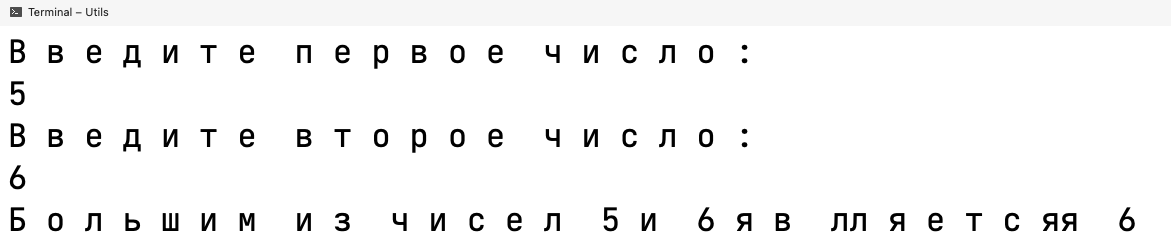
\includegraphics[width=0.7\textwidth]{images/task-1.png}
    \caption{Пример работы программы}
    \label{fig:task-1}
\end{figure}

\section{Использование в методах параметров, передаваемых по ссылке}

Выполнив все шаги из задания, я получил следующий код:

\inputminted{csharp}{../Utils/Utils/Utils1.cs}

\inputminted{csharp}{../Utils/Utils/Program1.cs}

На рис. \ref{fig:task-2} приведен пример работы программы.

\begin{figure}[H]
    \centering
    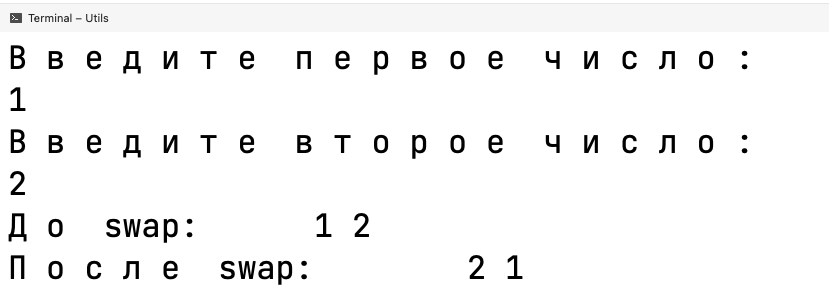
\includegraphics[width=0.7\textwidth]{images/task-2.png}
    \caption{Пример работы программы}
    \label{fig:task-2}
\end{figure}

\section{Использование возвращаемых параметров в методах}

Выполнив все шаги из задания, я получил следующий код:

\inputminted{csharp}{../Utils/Utils/Utils2.cs}

\inputminted{csharp}{../Utils/Utils/Program2.cs}

На рис. \ref{fig:task-3-1} и \ref{fig:task-3-2} приведен пример работы программы.

\begin{figure}[H]
    \centering
    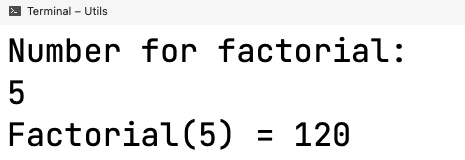
\includegraphics[width=0.5\textwidth]{images/task-3-1.png}
    \caption{Пример работы программы с небольшими значениями}
    \label{fig:task-3-1}
\end{figure}

\begin{figure}[H]
    \centering
    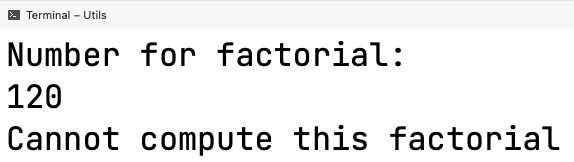
\includegraphics[width=0.5\textwidth]{images/task-3-2.png}
    \caption{Пример работы программы с значениями, вызывающими переполнение}
    \label{fig:task-3-2}
\end{figure}

\section{Расчет площади треугольника с помощью метода}

В методе \texttt{IsTriangle} я проверяю, что каждая сторона строго больше нуля, а также каждая сторона меньше суммы двух других сторон треугольника.

В методе \texttt{Square} для трех аргументов я сначала вызываю метод \texttt{IsTriangle}. Если пользователь передал некорректные данные, то функция выбрасывает исключение. После проверки я с помощью формулы Герона нахожу площадь треугольника.

В методе \texttt{Square} для одного аргумента я вызываю метод \texttt{Square} для трех аргументов, используя одну и ту же сторону в качестве аргументов. Исходный код программы приведен в следующем листинге:

\inputminted{csharp}{../Square/Square/Operation.cs}

В методе \texttt{main} я сначала спрашиваю у пользователя, какой тип треугольника использовать. После этого в зависимости от типа я считываю либо одну сторону, либо три стороны. Затем я вызываю метод \texttt{Square} и вывожу значение площади в стандартный вывод. Исходный код программы приведен в следующем листинге:

\inputminted{csharp}{../Square/Square/Program.cs}

На рис. \ref{fig:task-4-1} приведен пример расчета площади равностороннего треугольника.

\begin{figure}[H]
    \centering
    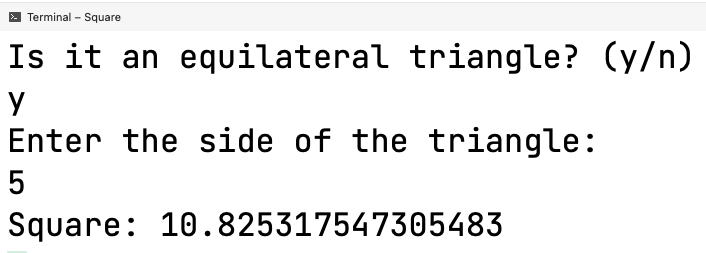
\includegraphics[width=0.6\textwidth]{images/task-4-1.png}
    \caption{Расчет площади равностороннего треугольника}
    \label{fig:task-4-1}
\end{figure}

На рис. \ref{fig:task-4-2} приведен пример расчета площади обычного треугольника.

\begin{figure}[H]
    \centering
    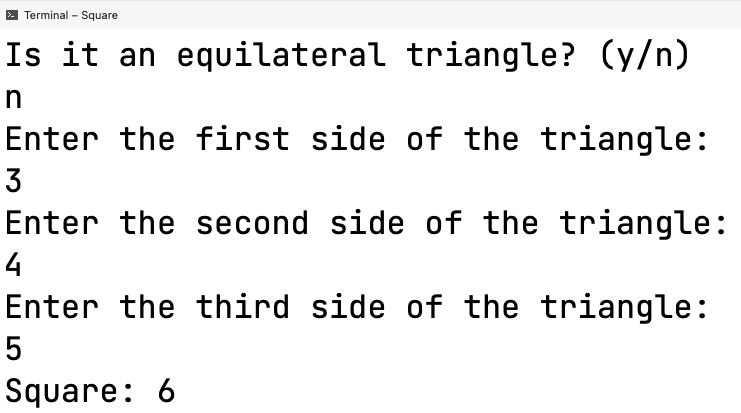
\includegraphics[width=0.6\textwidth]{images/task-4-2.png}
    \caption{Расчет площади обычного треугольника}
    \label{fig:task-4-2}
\end{figure}

На рис. \ref{fig:task-4-3} приведен пример расчета площади некорректного треугольника.

\begin{figure}[H]
    \centering
    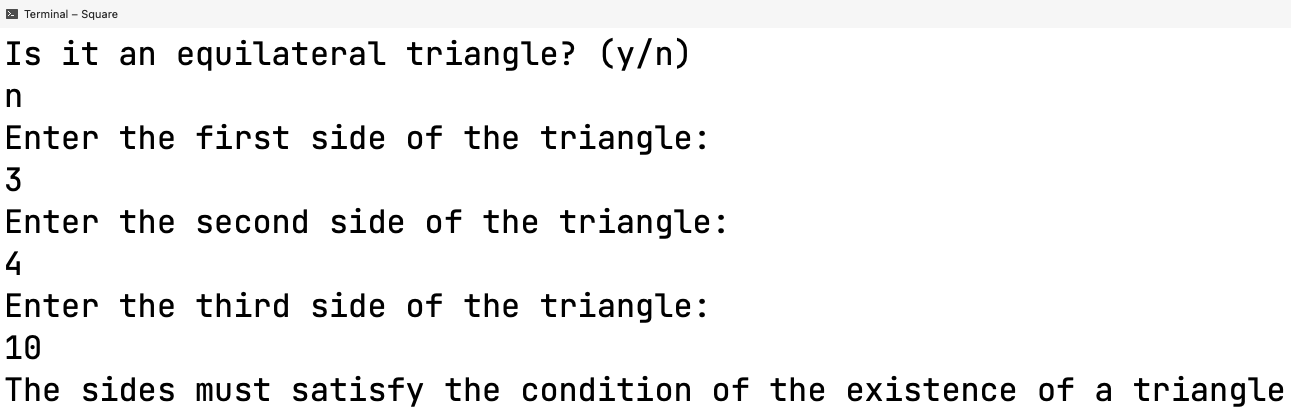
\includegraphics[width=0.7\textwidth]{images/task-4-3.png}
    \caption{Расчет площади некорректного треугольника}
    \label{fig:task-4-3}
\end{figure}

\section{Вычисление корней квадратного уравнения}

В методе \texttt{FindRoots} я нахожу дискриминант уравнения, после чего, в зависимости от значения дискриминанта я нахожу корни. Исходный код программы представлен в следующем листинге:
\inputminted{csharp}{../EquationRoots/EquationRoots/Equation.cs}

В методе \texttt{main} я сначала считываю значения параметров уравнения \texttt{a}, \texttt{b} и \texttt{c}, а после этого вызываю метод \texttt{FindRoots}. В зависимости от возвращаемого значения я вывожу ответ на экран. Исходный код программы представлен в следующем листинге:
\inputminted{csharp}{../EquationRoots/EquationRoots/Program.cs}

На рис. \ref{fig:task-5-1} показан пример выражения, не имеющего корней.

\begin{figure}[H]
    \centering
    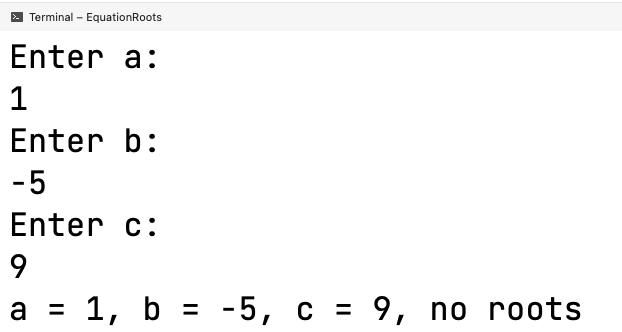
\includegraphics[width=0.5\textwidth]{images/task-5-1.png}
    \caption{Пример, не имеющий корней}
    \label{fig:task-5-1}
\end{figure}

На рис. \ref{fig:task-5-2} показан пример выражения, имеющего только один корень.

\begin{figure}[H]
    \centering
    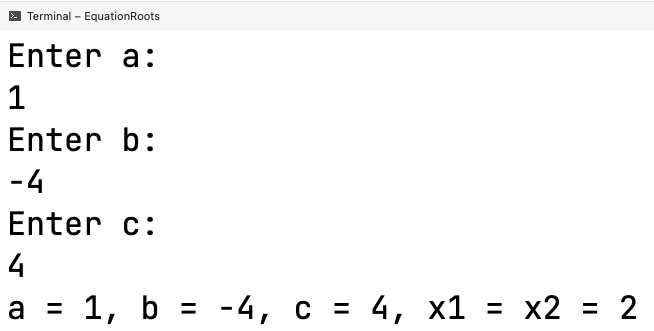
\includegraphics[width=0.5\textwidth]{images/task-5-2.png}
    \caption{Пример, имеющий только один корень}
    \label{fig:task-5-2}
\end{figure}

На рис. \ref{fig:task-5-3} показан пример выражения, имеющего два корня.

\begin{figure}[H]
    \centering
    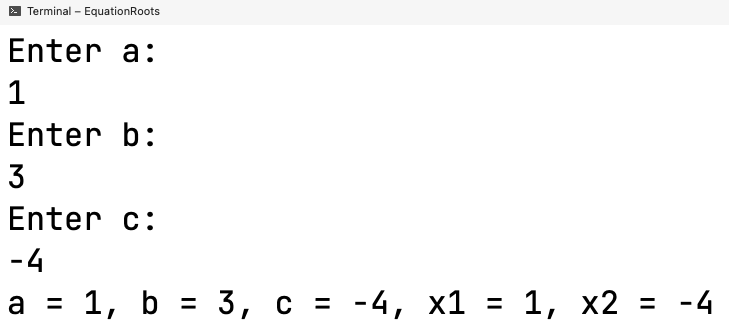
\includegraphics[width=0.5\textwidth]{images/task-5-3.png}
    \caption{Пример, имеющий два корня}
    \label{fig:task-5-3}
\end{figure}

\end{document}
